\section{Sichuan Pepper}
\label{sec:sichuan_pepper}

\begin{spice}\label{spice:Sichuan pepper}
\textsc{Sichuan pepper} \hfill \href{https://powo.science.kew.org/taxon/775625-1}{POWO} \\
\textbf{English:} \textit{Sichuan pepper}. 
\textbf{Arabic:} {\arabicfont{فلفل سيتشوان}} \textit{fulful sītshuwān} [Sichuan pepper]. 
\textbf{Chinese:} {\tradchinesefont{花椒}} \textit{huā​jiāo} [flower-pepper]. 
\textbf{Hungarian:} \textit{szecsuáni bors} [Sichuan pepper].  \\
\noindent{\color{black}\rule[0.5ex]{\linewidth}{.5pt}}
\begin{tabular}{@{}p{0.25\linewidth}@{}p{0.75\linewidth}@{}}
Plant species: & \taxonn{Zanthoxylum bungeanum}{Maxim.}; \textit{\taxonn{Z. armatum}{DC.}; et al.} \\
Family: & \textit{Rutaceae} \\
part used: & pericarp \\
Region of origin: & China \\
Cultivated in: & China \\
Color: & red; green \\
\end{tabular}
\end{spice}

\begin{figure}[!ht]
	\vspace{-4ex}
	\centering
	\subfloat[\centering a]{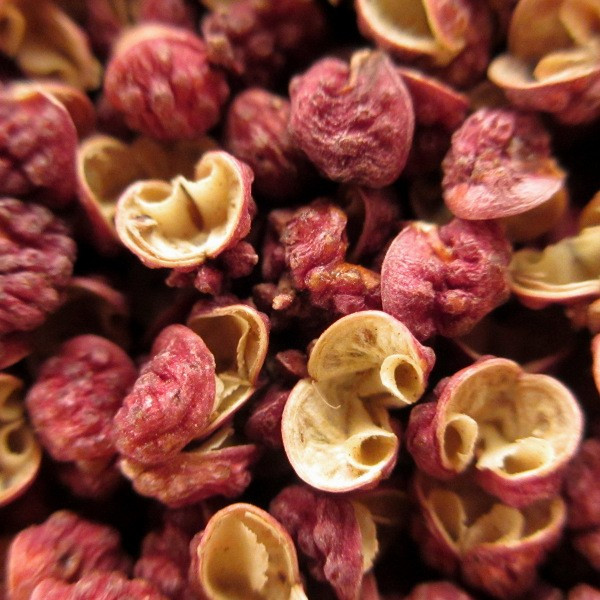
\includegraphics[width=0.3\linewidth]{imgs/spices/sichuan_pepper-1.jpg}}
	\hfill
	\subfloat[\centering b]{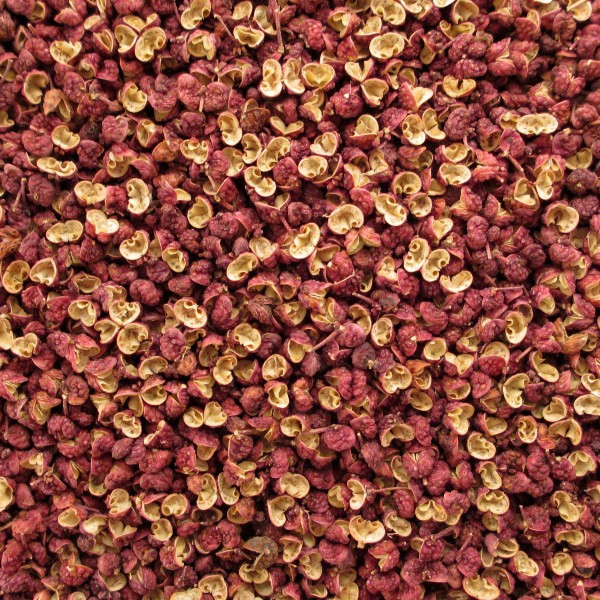
\includegraphics[width=0.3\linewidth]{imgs/spices/sichuan_pepper-2.jpg}}
	\hfill
	\subfloat[\centering c]{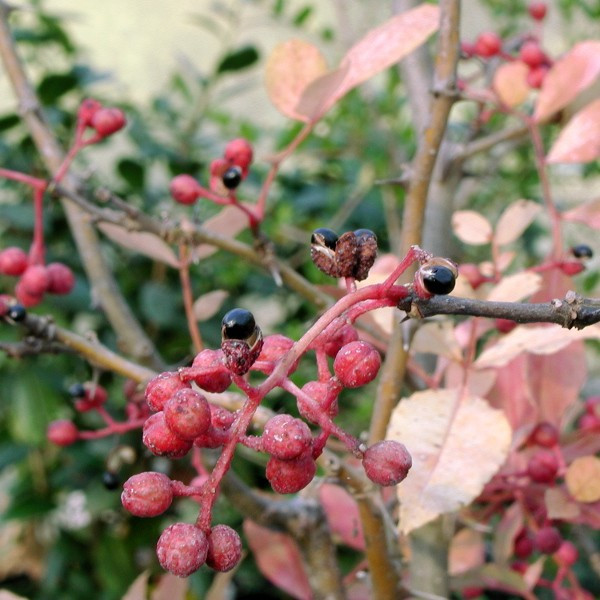
\includegraphics[width=0.3\linewidth]{imgs/spices/sichuan_pepper-3.jpg}}
	\caption{Sichuan Pepper \taxon{}.}
	\label{fig:sichuan_pepper_imgs}
\end{figure}

\subsection{The Botany, Origins, and Cultivation of Sichuan Pepper}

\subsection{The History of Sichuan Pepper}

\subsection{The Names of Sichuan Pepper}

\subsubsection{English}

\begin{table}[!ht]
    \caption{Various names for Sichuan pepper in English.}
\centering
\begin{tabularx}{\textwidth}{@{}l>{\itshape \small}lL>{\small}l@{}}
\toprule
\textbf{\#} & \multicolumn{1}{l}{\textbf{Species}} & \multicolumn{1}{l}{\textbf{Name}} & \multicolumn{1}{l}{\textbf{Source}} \\
\midrule
1	& Z. bungeanum; Z. armatum; Z. simulans	& Chinese pepper	& \textcite{davis_vocabulary_1824} \\
2	& Zanthoxilum schinifolium	& sancho	& \textcite{van_wyk_culinary_2014} \\
3	& Zanthoxylum ailanthoides	& yue jiao	& \textcite{van_wyk_culinary_2014} \\
4	& Zanthoxylum alatum	& timut	& \textcite{van_wyk_culinary_2014} \\
5	& Zanthoxylum armatum	& Nepal pepper	& \textcite{austin_sichuan_2008} \\
6	& Zanthoxylum armatum	& winged prickly ash	&  \\
7	& Zanthoxylum armatum	& zhu ye jiao	& \textcite{van_wyk_culinary_2014} \\
8	& Zanthoxylum piperitum	& anise pepper	& \textcite{austin_sichuan_2008} \\
9	& Zanthoxylum piperitum	& Japanese pepper	& \textcite{van_wyk_culinary_2014} \\
10	& Zanthoxylum piperitum	& Japanese prickly-ash	&  \\
11	& Zanthoxylum piperitum	& sansho	& \textcite{van_wyk_culinary_2014} \\
12	& Zanthoxylum simulans	& chuan jiao	& \textcite{van_wyk_culinary_2014} \\
13	& Zanthoxylum spp.	& brown pepper	& \textcite{austin_sichuan_2008} \\
14	& Zanthoxylum spp.	& Chinese prickly ash	&  \\
15	& Zanthoxylum spp.	& fagara	& \textcite{austin_sichuan_2008} \\
16	& Zanthoxylum spp.	& prickly ash	& \textcite{oed} \\
\textbf{17}	& \textbf{Zanthoxylum spp.}	& \textbf{Sichuan pepper}	& \textbf{\textcite{van_wyk_culinary_2014}} \\
\bottomrule
\end{tabularx}
\label{table:names_Sichuan_pepper_en}
\end{table}



\subsubsection{Arabic}

\begin{table}[!ht]
\centering
\begin{tabularx}{\textwidth}{@{}l>{\itshape \small}lr>{\itshape}lL>{\small}l@{}}
\toprule
\textbf{\#} & \multicolumn{1}{l}{\textbf{Species}} & \multicolumn{1}{l}{\textbf{Name}} & \multicolumn{1}{l}{\textbf{Tr.}} & \multicolumn{1}{l}{\textbf{Gloss}} & \multicolumn{1}{l}{\textbf{Source}} \\
\midrule
\textbf{1}	& \textbf{Zanthoxylum spp.}	& \textbf{فلفل سيتشوان}	& \textbf{fulful sītshuwān}	& \textbf{Sichuan pepper}	& \textbf{\textcite{wikipedia}} \\
2	& Zanthoxylum spp.	& فاغرة	& fāghira 	& 	& \textcite{lane_arabic-english_1863} \\
\bottomrule
\end{tabularx}
\caption{Various names for Sichuan pepper in Arabic.}
\label{table:names_Sichuan_pepper_ar}
\end{table}



\subsubsection{Chinese}

\begin{table}[!ht]
\centering
\begin{tabularx}{\textwidth}{@{}l>{\itshape \small}ll>{\itshape}lL>{\small}l@{}}
\toprule
\textbf{\#} & \multicolumn{1}{l}{\textbf{Species}} & \multicolumn{1}{l}{\textbf{Name}} & \multicolumn{1}{l}{\textbf{Tr.}} & \multicolumn{1}{l}{\textbf{Gloss}} & \multicolumn{1}{l}{\textbf{Source}} \\
\midrule
1	& Zanthoxylum armatum	& \traditionalchinesefont{竹葉椒}	& zhúyèjiāo	& bamboo-leaf-pepper	&  \\
\textbf{2}	& \textbf{Zanthoxylum bungeanum}	& \textbf{\traditionalchinesefont{花椒}}	& \textbf{huā​jiāo}	& \textbf{flower-pepper}	& \textbf{\textcite{hu_food_2005}} \\
3	& Zanthoxylum piperitum	& \traditionalchinesefont{日本花椒}	& rìběn huājiāo	& Japanese-flower-pepper	&  \\
4	& Zanthoxylum piperitum	& \traditionalchinesefont{山椒}	& shānjiāo	& mountain-pepper	& \textcite{wikipedia} \\
5	& Zanthoxylum schinifolium	& \traditionalchinesefont{青花椒}	& qīnghuājiāo	& green-flower-pepper	& \textcite{hu_food_2005} \\
6	& Zanthoxylum schinifolium	& \traditionalchinesefont{香椒子}	& xiāngjiāozi	& fragrant-pepper-seed	& \textcite{hu_food_2005} \\
7	& Zanthoxylum schinifolium	& \traditionalchinesefont{崖椒}	& yájiāo	& cliff-pepper	& \textcite{hu_food_2005} \\
8	& Zanthoxylum simulans?	& \traditionalchinesefont{川椒}	& chuānjiāo	& river(=Sichuan)-pepper	& \textcite{hu_food_2005} \\
9	& Zanthoxylum spp.	& \traditionalchinesefont{椒}	& jiāo	& pepper	& \textcite{defrancis_abc_2003} \\
10	& Zanthoxylum spp.	& \traditionalchinesefont{麻椒}	& má​jiāo	& numbing-pepper	&  \\
11	& Zanthoxylum spp.	& \traditionalchinesefont{蜀椒}	& shǔjiāo 	& Sichuan-pepper	& \textcite{wikipedia} \\
\bottomrule
\end{tabularx}
\caption{Various names for Sichuan pepper in Chinese.}
\label{table:names_Sichuan_pepper_zh}
\end{table}



\subsubsection{Summary}

\begin{table}[!ht]
\centering
\begin{tabularx}{\textwidth}{@{}ll>{\itshape}lLl>{\small}l@{}}
\toprule
\textbf{\#} & \textbf{Language} & \multicolumn{1}{l}{\textbf{Term}} & \textbf{Gloss} & \textbf{Loan} & \multicolumn{1}{l}{\textbf{Source}} \\
\midrule
1	& English	& Chinese pepper	& 	& no	& \textcite{oed} \\
2	& English	& Japanese pepper	& 	& no	& \textcite{oed} \\
3	& English	& prickly ash	& 	& no	& \textcite{oed} \\
\midrule
\midrule
1	& Chinese	& huā​jiāo	& flower-pepper	& no	& \textcite{defrancis_abc_2003} \\
2	& Chinese	& jiāo	& pepper	& no	& \textcite{defrancis_abc_2003} \\
\bottomrule
\end{tabularx}
\caption{Conventionalized names for Sichuan pepper in English, Arabic, and Chinese, found in dictionaries.}
\label{table:names_Sichuan_pepper}
\end{table}








% EE:

% OE:

% MW:

% AH:

% WK:
